\section{Results}
\label{sect:results}

\subsection{Experimental Design}
\label{subsect:experimental-design}

Experiments ran on an Intel Core i5-7200U, 8 GB RAM, Ubuntu 22.04 64-bit, with an NVIDIA GeForce GT 940MX GPU.

We used classical volume ray-casting with Blinn-Phong illumination and trilinear interpolation. Ray step adjusted per voxel spacing. Runtimes are averages of five trials.

The system was implemented in C++ using Qt and CUDA C/C++. The implementation is publicly available.

Table~\ref{tab:datasets-descriptions} lists the volume datasets used in experiments.

All volumes contain scalar density values. Multidimensional attributes were derived—13 in total—including intensity, gradient magnitude, Laplacian magnitude, and 10 local histogram statistics (absolute deviation, contrast, energy, entropy, inertia, kurtosis, mean, skewness, standard deviation, variance).

Attribute selection was empirical, tailored per dataset to balance discrimination and computational cost.

\begin{table}[htb!]
    \centering
    \caption{Volume datasets.}
    \begin{tabular}{@{}ccc@{}}
        \toprule
        \textbf{Dataset} & \textbf{Grid size} & \textbf{Total voxels} \\ 
        \midrule
        Engine block & $256 \times 256 \times 256$ & 16,777,216\\
        Knees & $379 \times 229 \times 305$ & 26,471,255\\
        Tooth & $256 \times 256 \times 161$ & 10,551,296\\
        \bottomrule
        \label{tab:datasets-descriptions}
    \end{tabular}
\end{table}

\subsection{Runtime}
\label{subsect:runtime-analysis}

Table~\ref{tab:runtime-analysis} presents runtimes (seconds) for each dataset.

\begin{table}[!htbp]
\caption{Runtime (seconds) of the proposed method per dataset.}
\label{tab:runtime-analysis}
\centering
    \begin{tabular}{@{}>{\centering\arraybackslash}m{0.4\columnwidth}>{\centering\arraybackslash}m{0.15\columnwidth}>{\centering\arraybackslash}m{0.15\columnwidth}>{\centering\arraybackslash}m{0.15\columnwidth}@{}}
        \toprule
            & \textbf{Engine block} & \textbf{Knees} & \textbf{Tooth}\\
        \midrule
        \textbf{Dimensionality reduction} & 7.50 & 7.98 & 36.05 \\
        \textbf{Clustering} & 51.52 & 102.77 & 19.42 \\
        \textbf{Pivot-based indexing} & 2.23 & 3.15 & 1.33 \\
        \midrule
        \textbf{Volume exploration space} & 1.48 & 1.86 & 0.79 \\
        \bottomrule
    \end{tabular}
\end{table}

\subsection{Data classification}
\label{subsect:material-classification}

Attribute selection was done empirically by iterative testing and visual assessment, ensuring effective separation of volumetric structures while maintaining computational feasibility.

DBSCAN's $minPts$ was fixed at 4~\cite{ester1996}. Parameter $\varepsilon$ varied within $[0.2, 0.35]$, and SSS parameter $\alpha$ within $[0.8, 0.95]$ for volume exploration.

\subsubsection{Engine block dataset}
\label{subsubsec:engine-block}

Figure~\ref{fig:engine-block-clusters-tf} shows the volume exploration space for the engine block. Each numbered group corresponds to classified volume details in Fig.~\ref{fig:engine-block-clusters}. Parameters: $k=4$, TF = \{intensity, skewness, gradient magnitude, variance\}; $minPts=4$; $\varepsilon=0.35$; $\alpha=0.85$.

\begin{figure}[htb!]
    \centering
    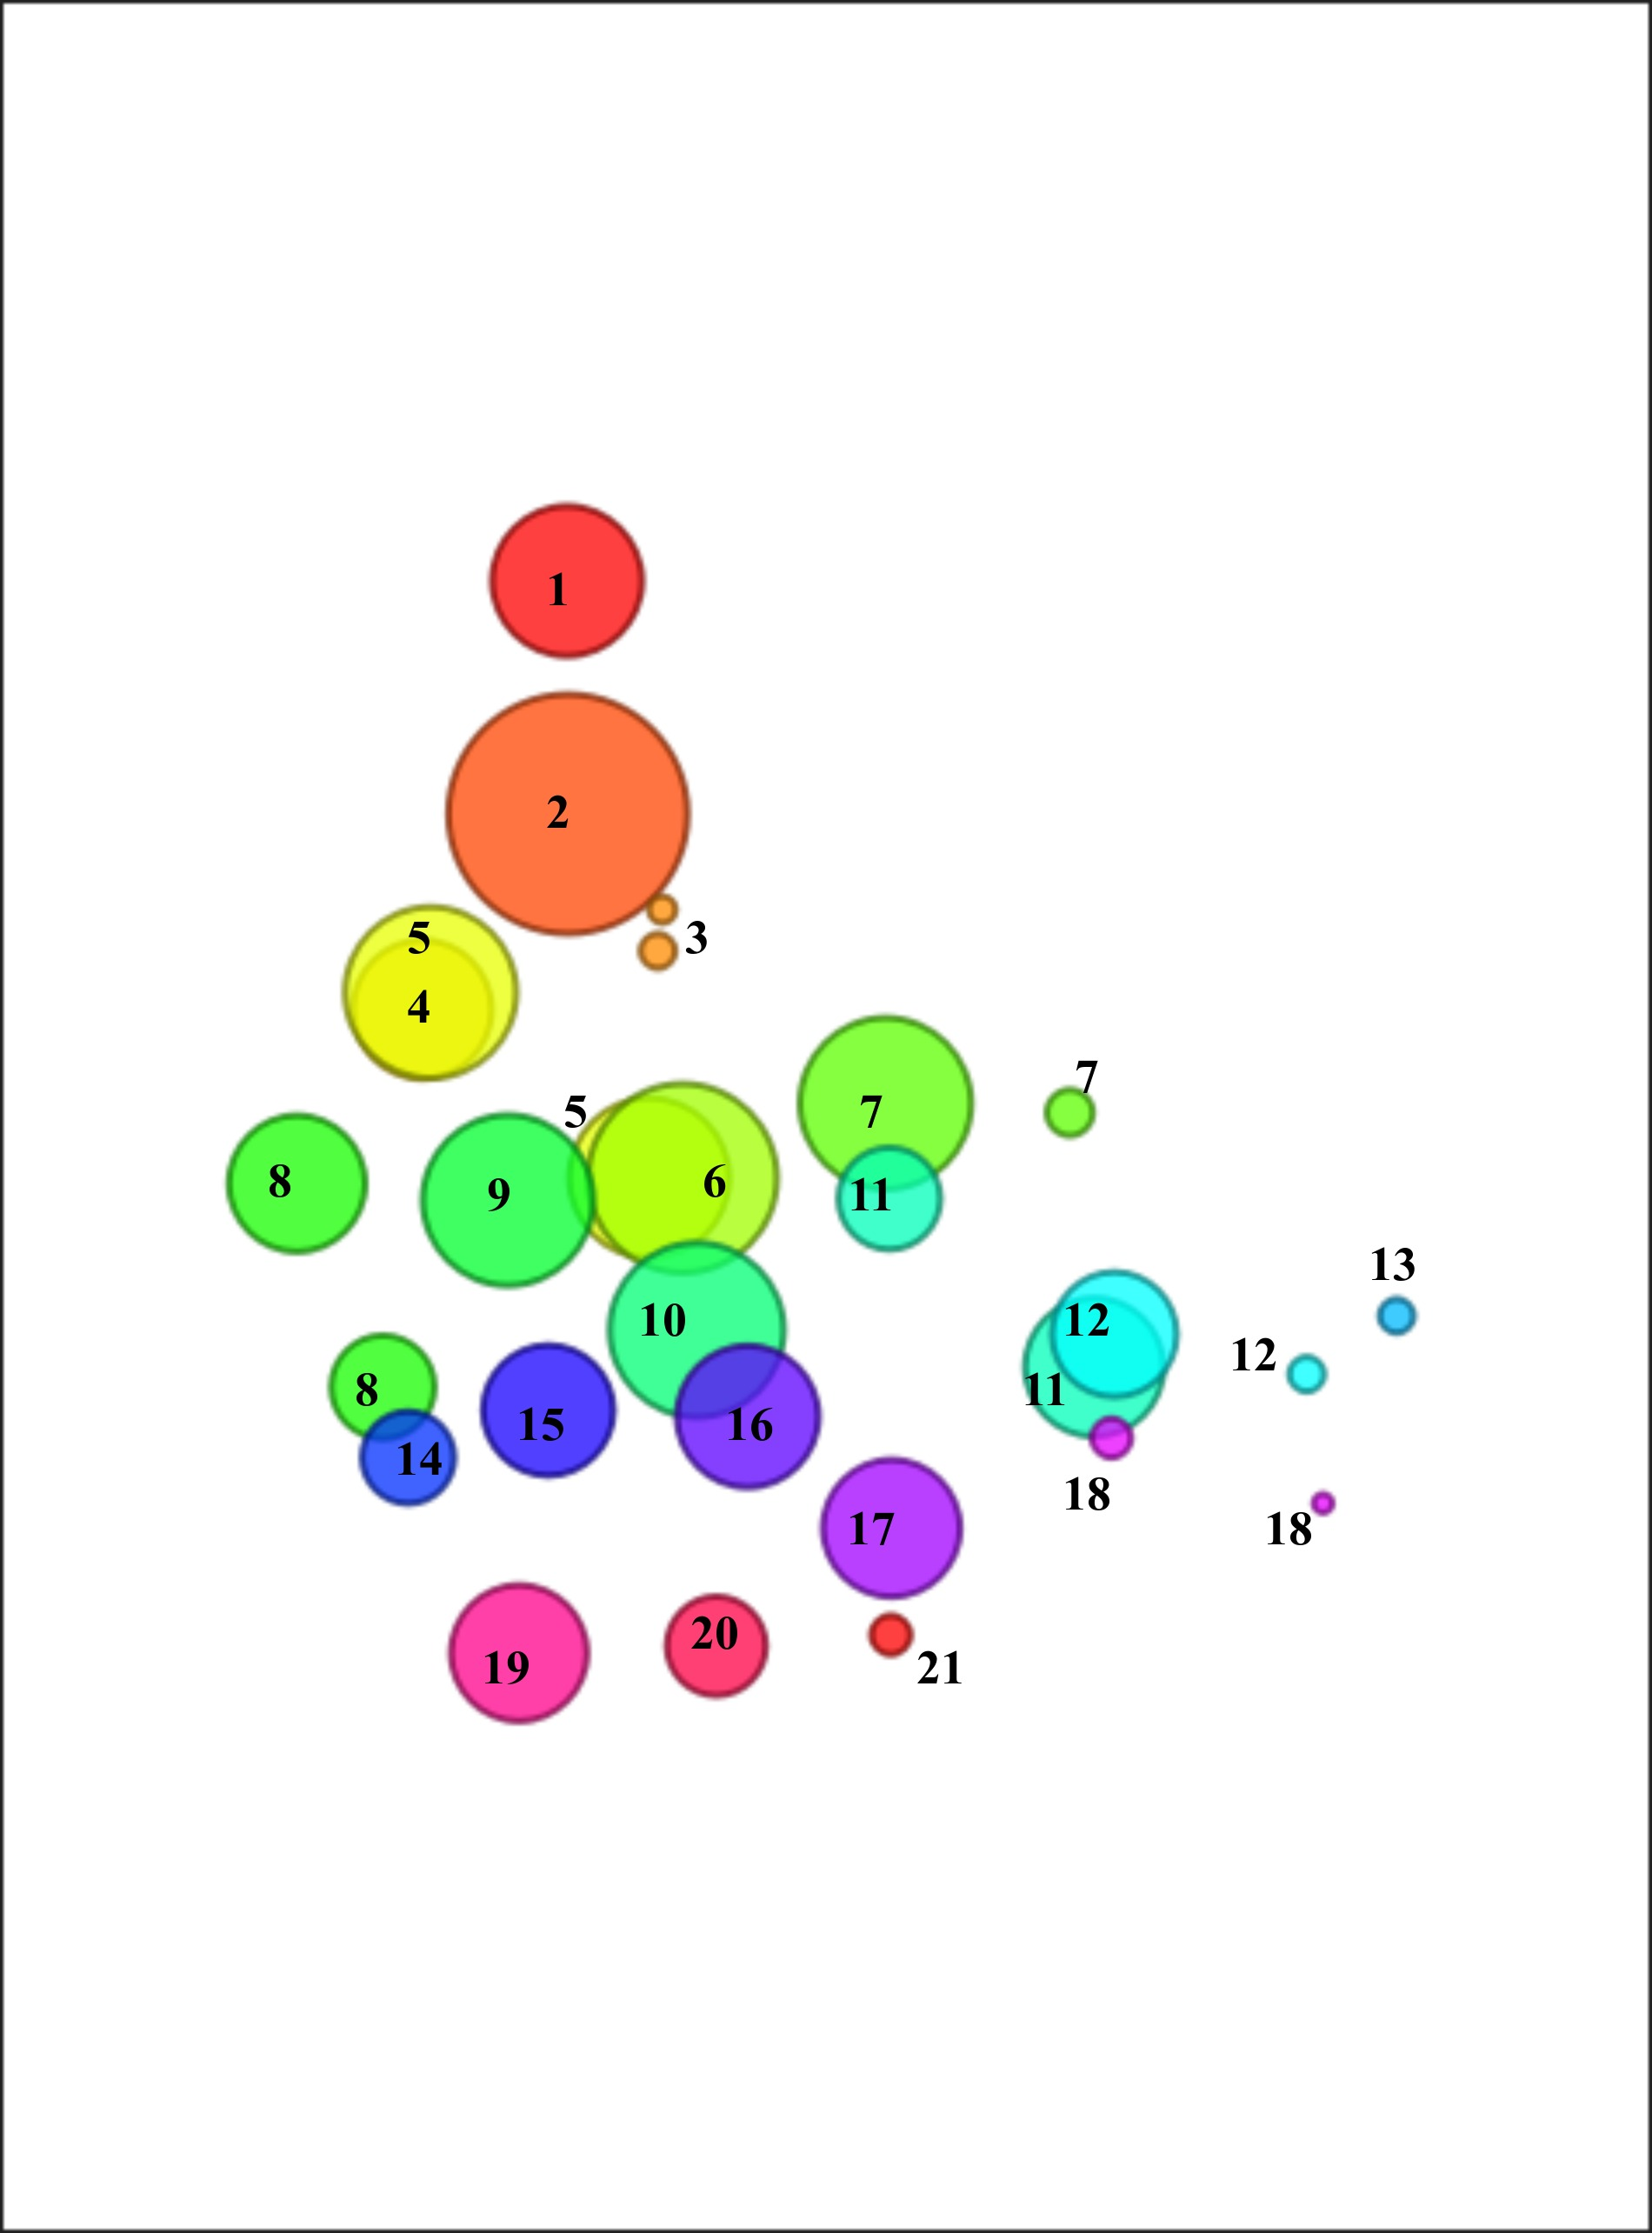
\includegraphics[width=0.7\columnwidth]{figs/engine-block-clusters-tf.jpg}
    \caption{Volume exploration space for engine block dataset. Parameters: TF = \{intensity, skewness, gradient magnitude, variance\}; $minPts=4$; $\varepsilon=0.35$; $\alpha=0.85$.}
    \label{fig:engine-block-clusters-tf}
\end{figure}

\begin{figure}[htb!]
    \centering
    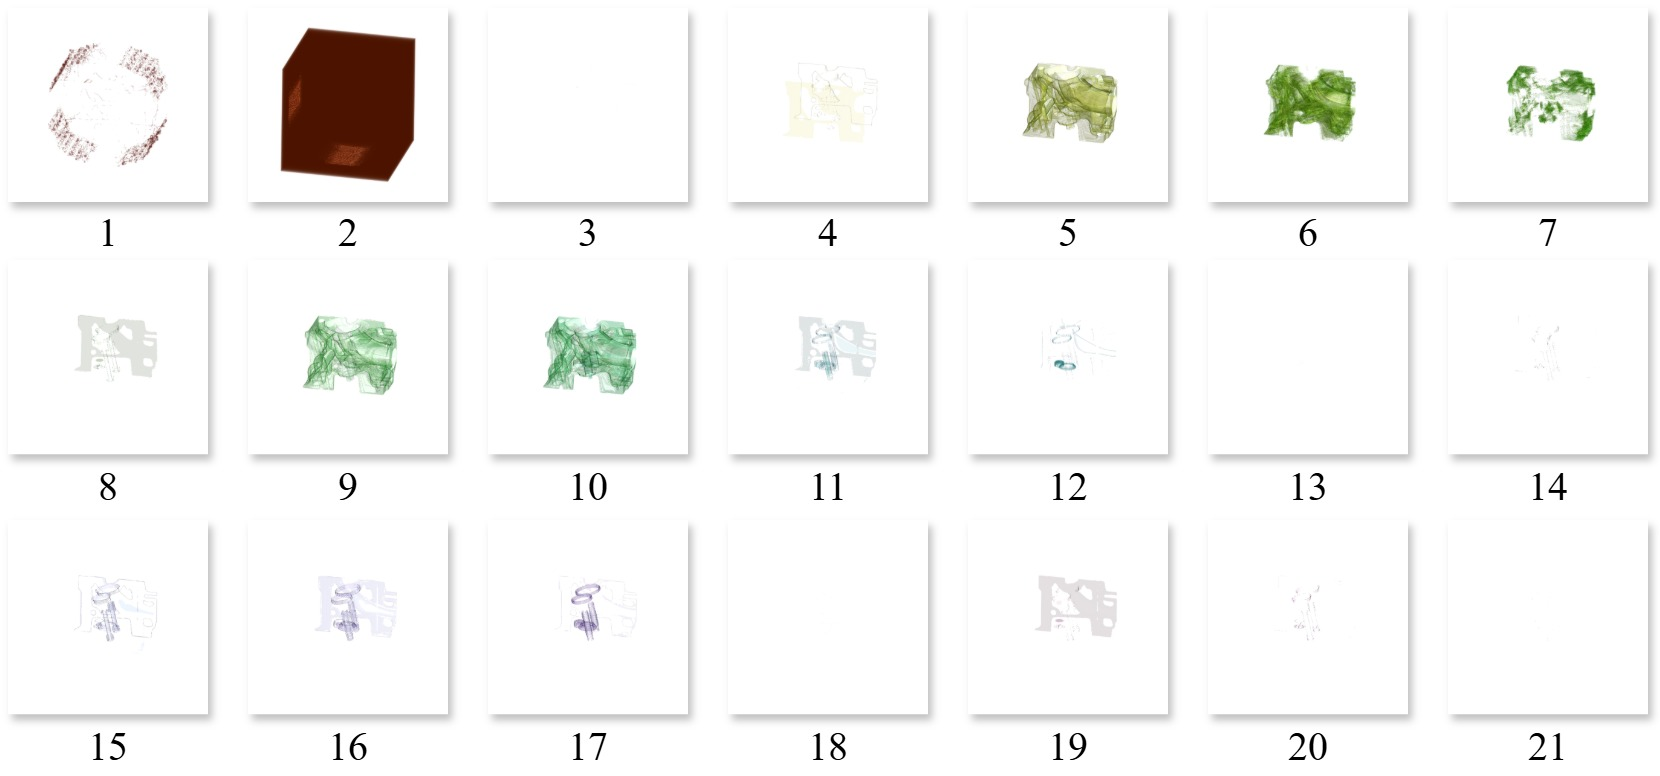
\includegraphics[width=\columnwidth]{figs/engine-block-clusters.jpg}
    \caption{Rendered classified volume details for engine block. Parameters as in Fig.~\ref{fig:engine-block-clusters-tf}.}
    \label{fig:engine-block-clusters}
\end{figure}

Figure~\ref{fig:engine-block-groups} shows a volume exploration simulation revealing engine components, starting from Fig.~\ref{fig:engine-block-clusters-tf}.

\begin{figure}[htb!]
    \centering
    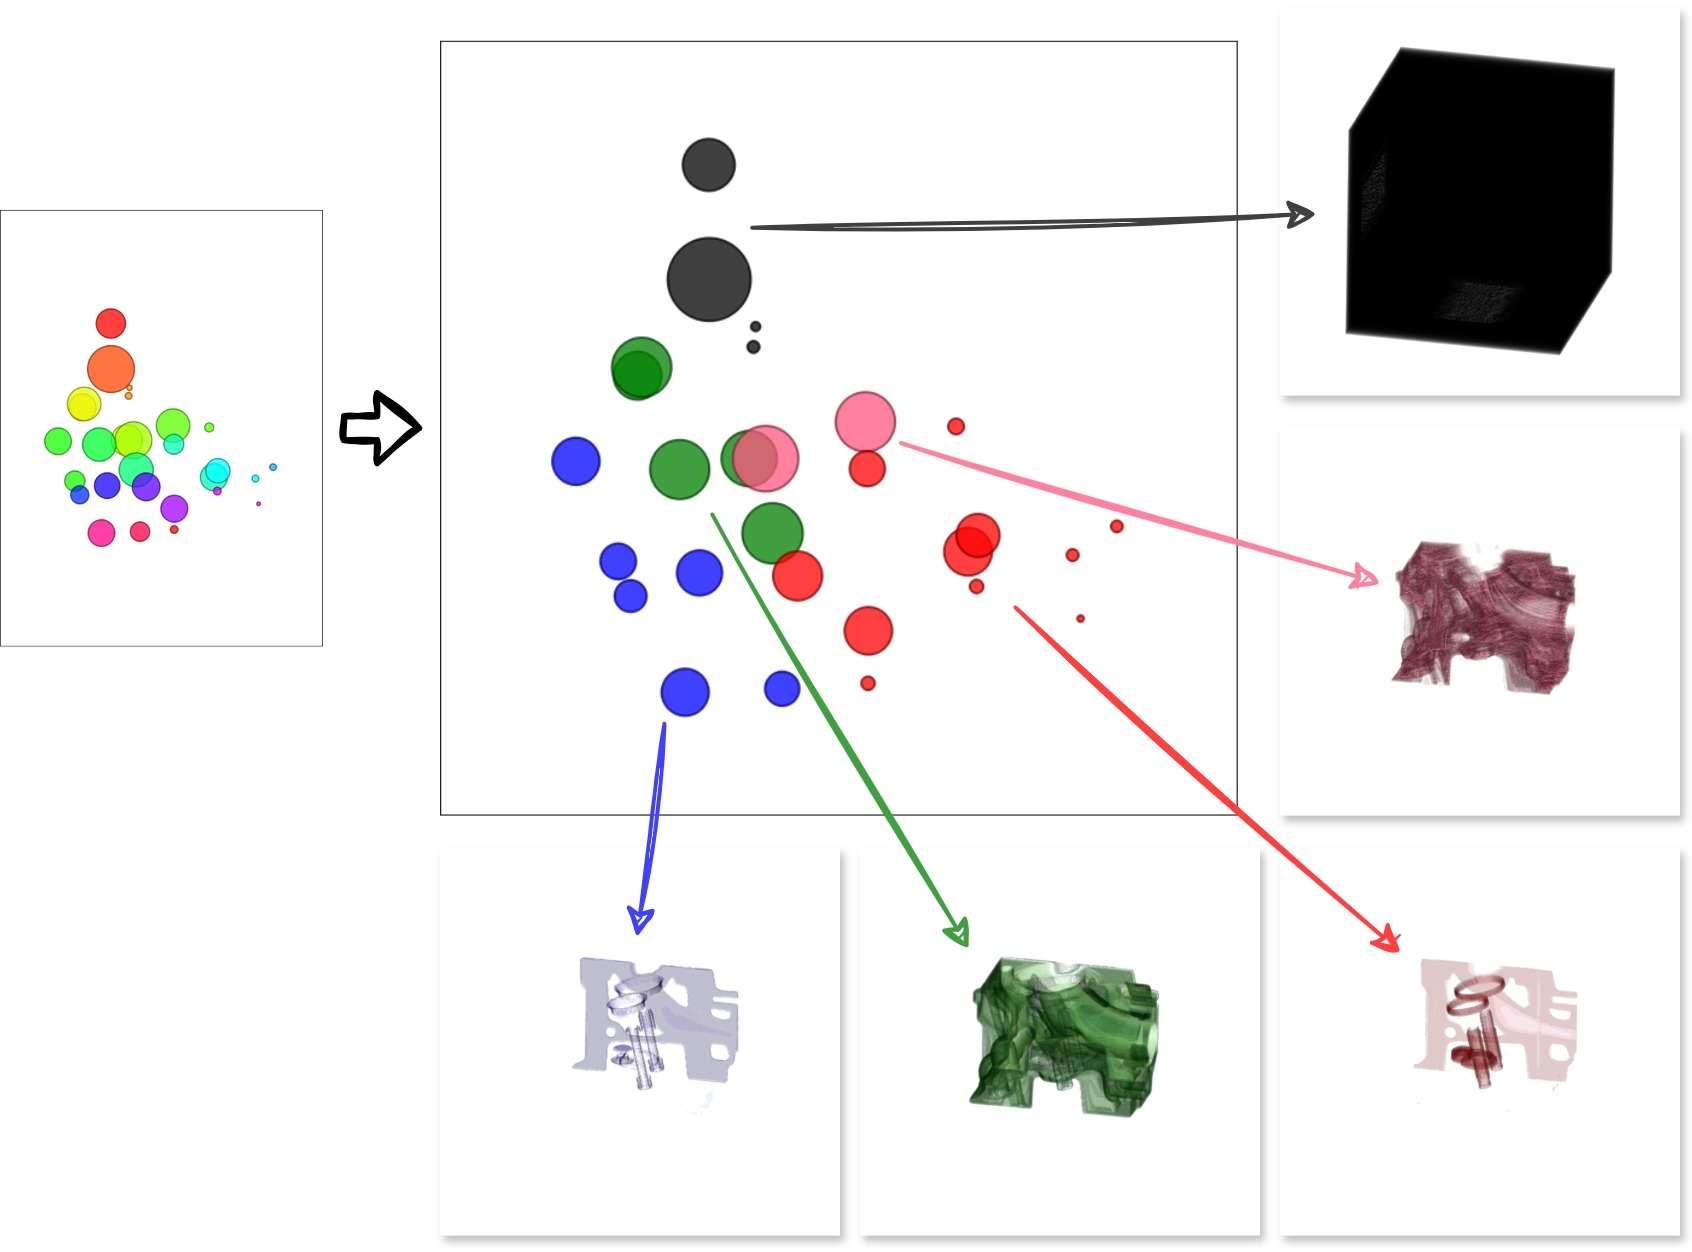
\includegraphics[width=\columnwidth]{figs/engine-block-groups.jpg}
    \caption{User-refined transfer function and volume classification for engine block. Groups formed empirically. Parameters as in Fig.~\ref{fig:engine-block-clusters-tf}.}
    \label{fig:engine-block-groups}
\end{figure}

\subsubsection{Knees dataset}
\label{subsubsect:knees-dataset}

Preliminary classification is shown in Fig.~\ref{fig:knees-tf-clusters} with rendered details in Fig.~\ref{fig:knees-clusters}. Parameters: TF = \{intensity, variance, absolute deviation, energy, contrast\}; $minPts=4$; $\varepsilon=0.35$; $\alpha=0.9$.

\begin{figure}[htb!]
    \centering
    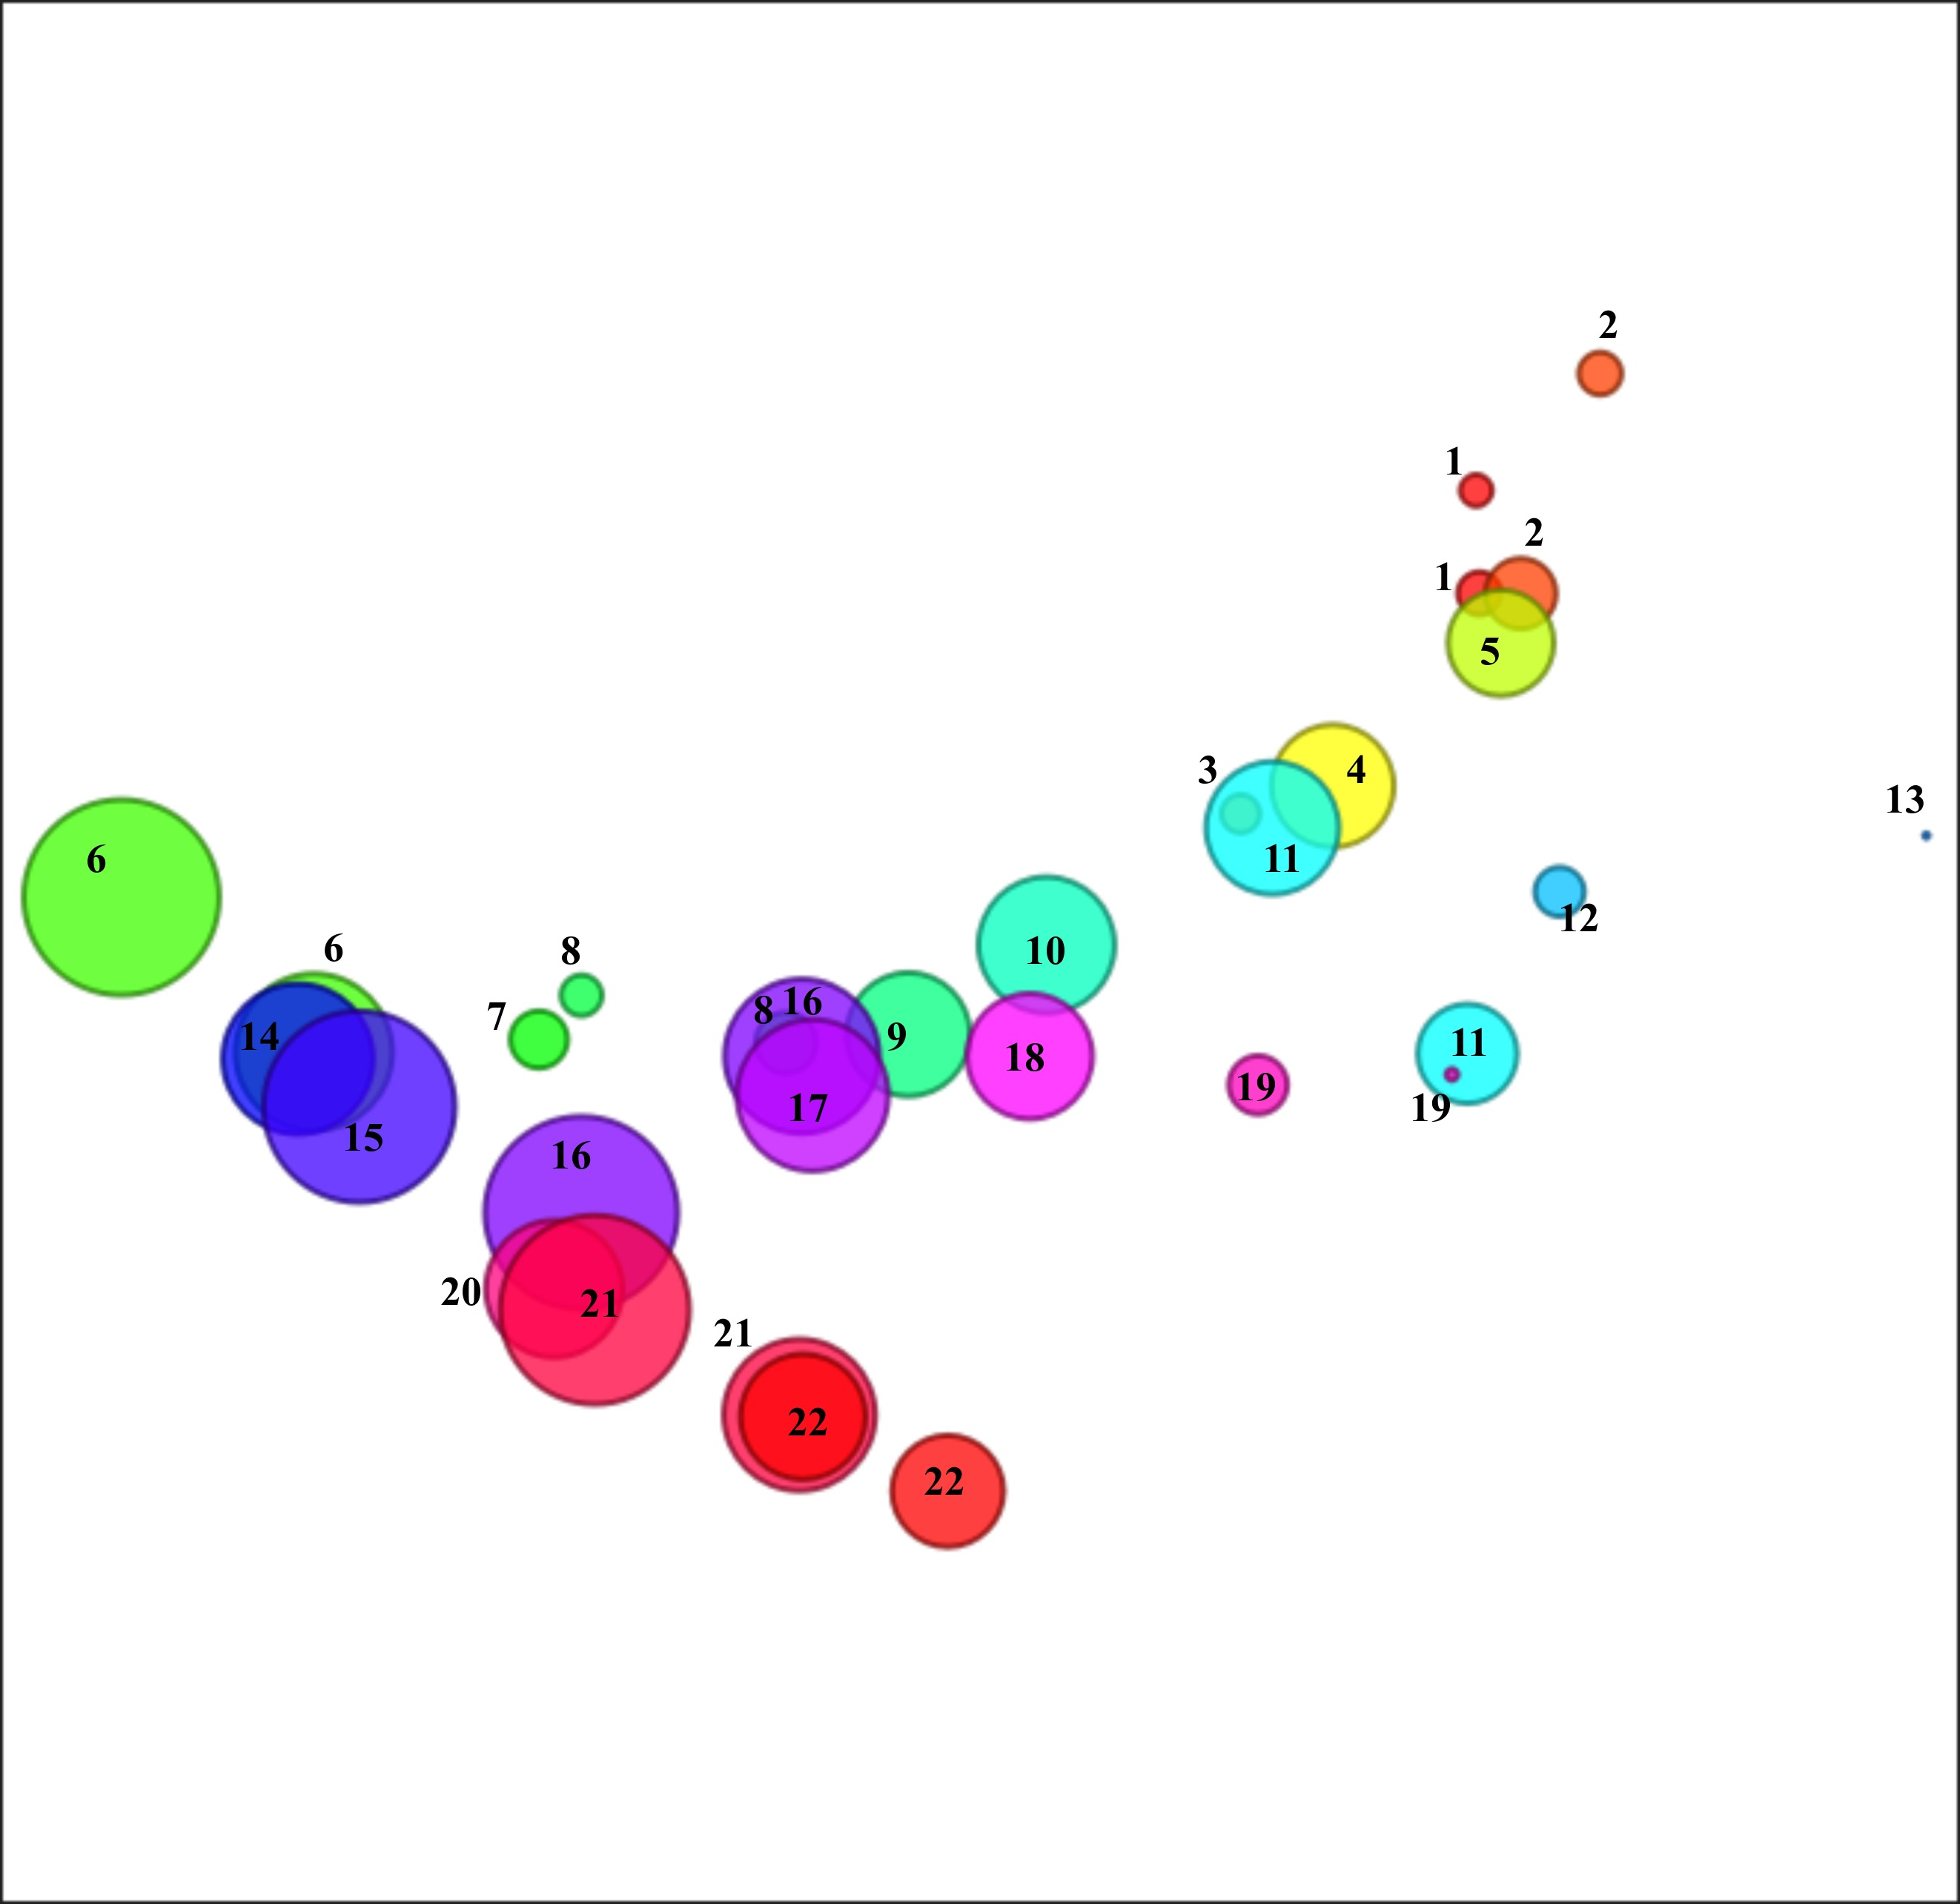
\includegraphics[width=0.7\columnwidth]{figs/knees-clusters-tf.jpg} 
    \caption{Volume exploration space for knees dataset. Parameters as above.}
    \label{fig:knees-tf-clusters}
\end{figure}

\begin{figure}[htb!]
    \centering
    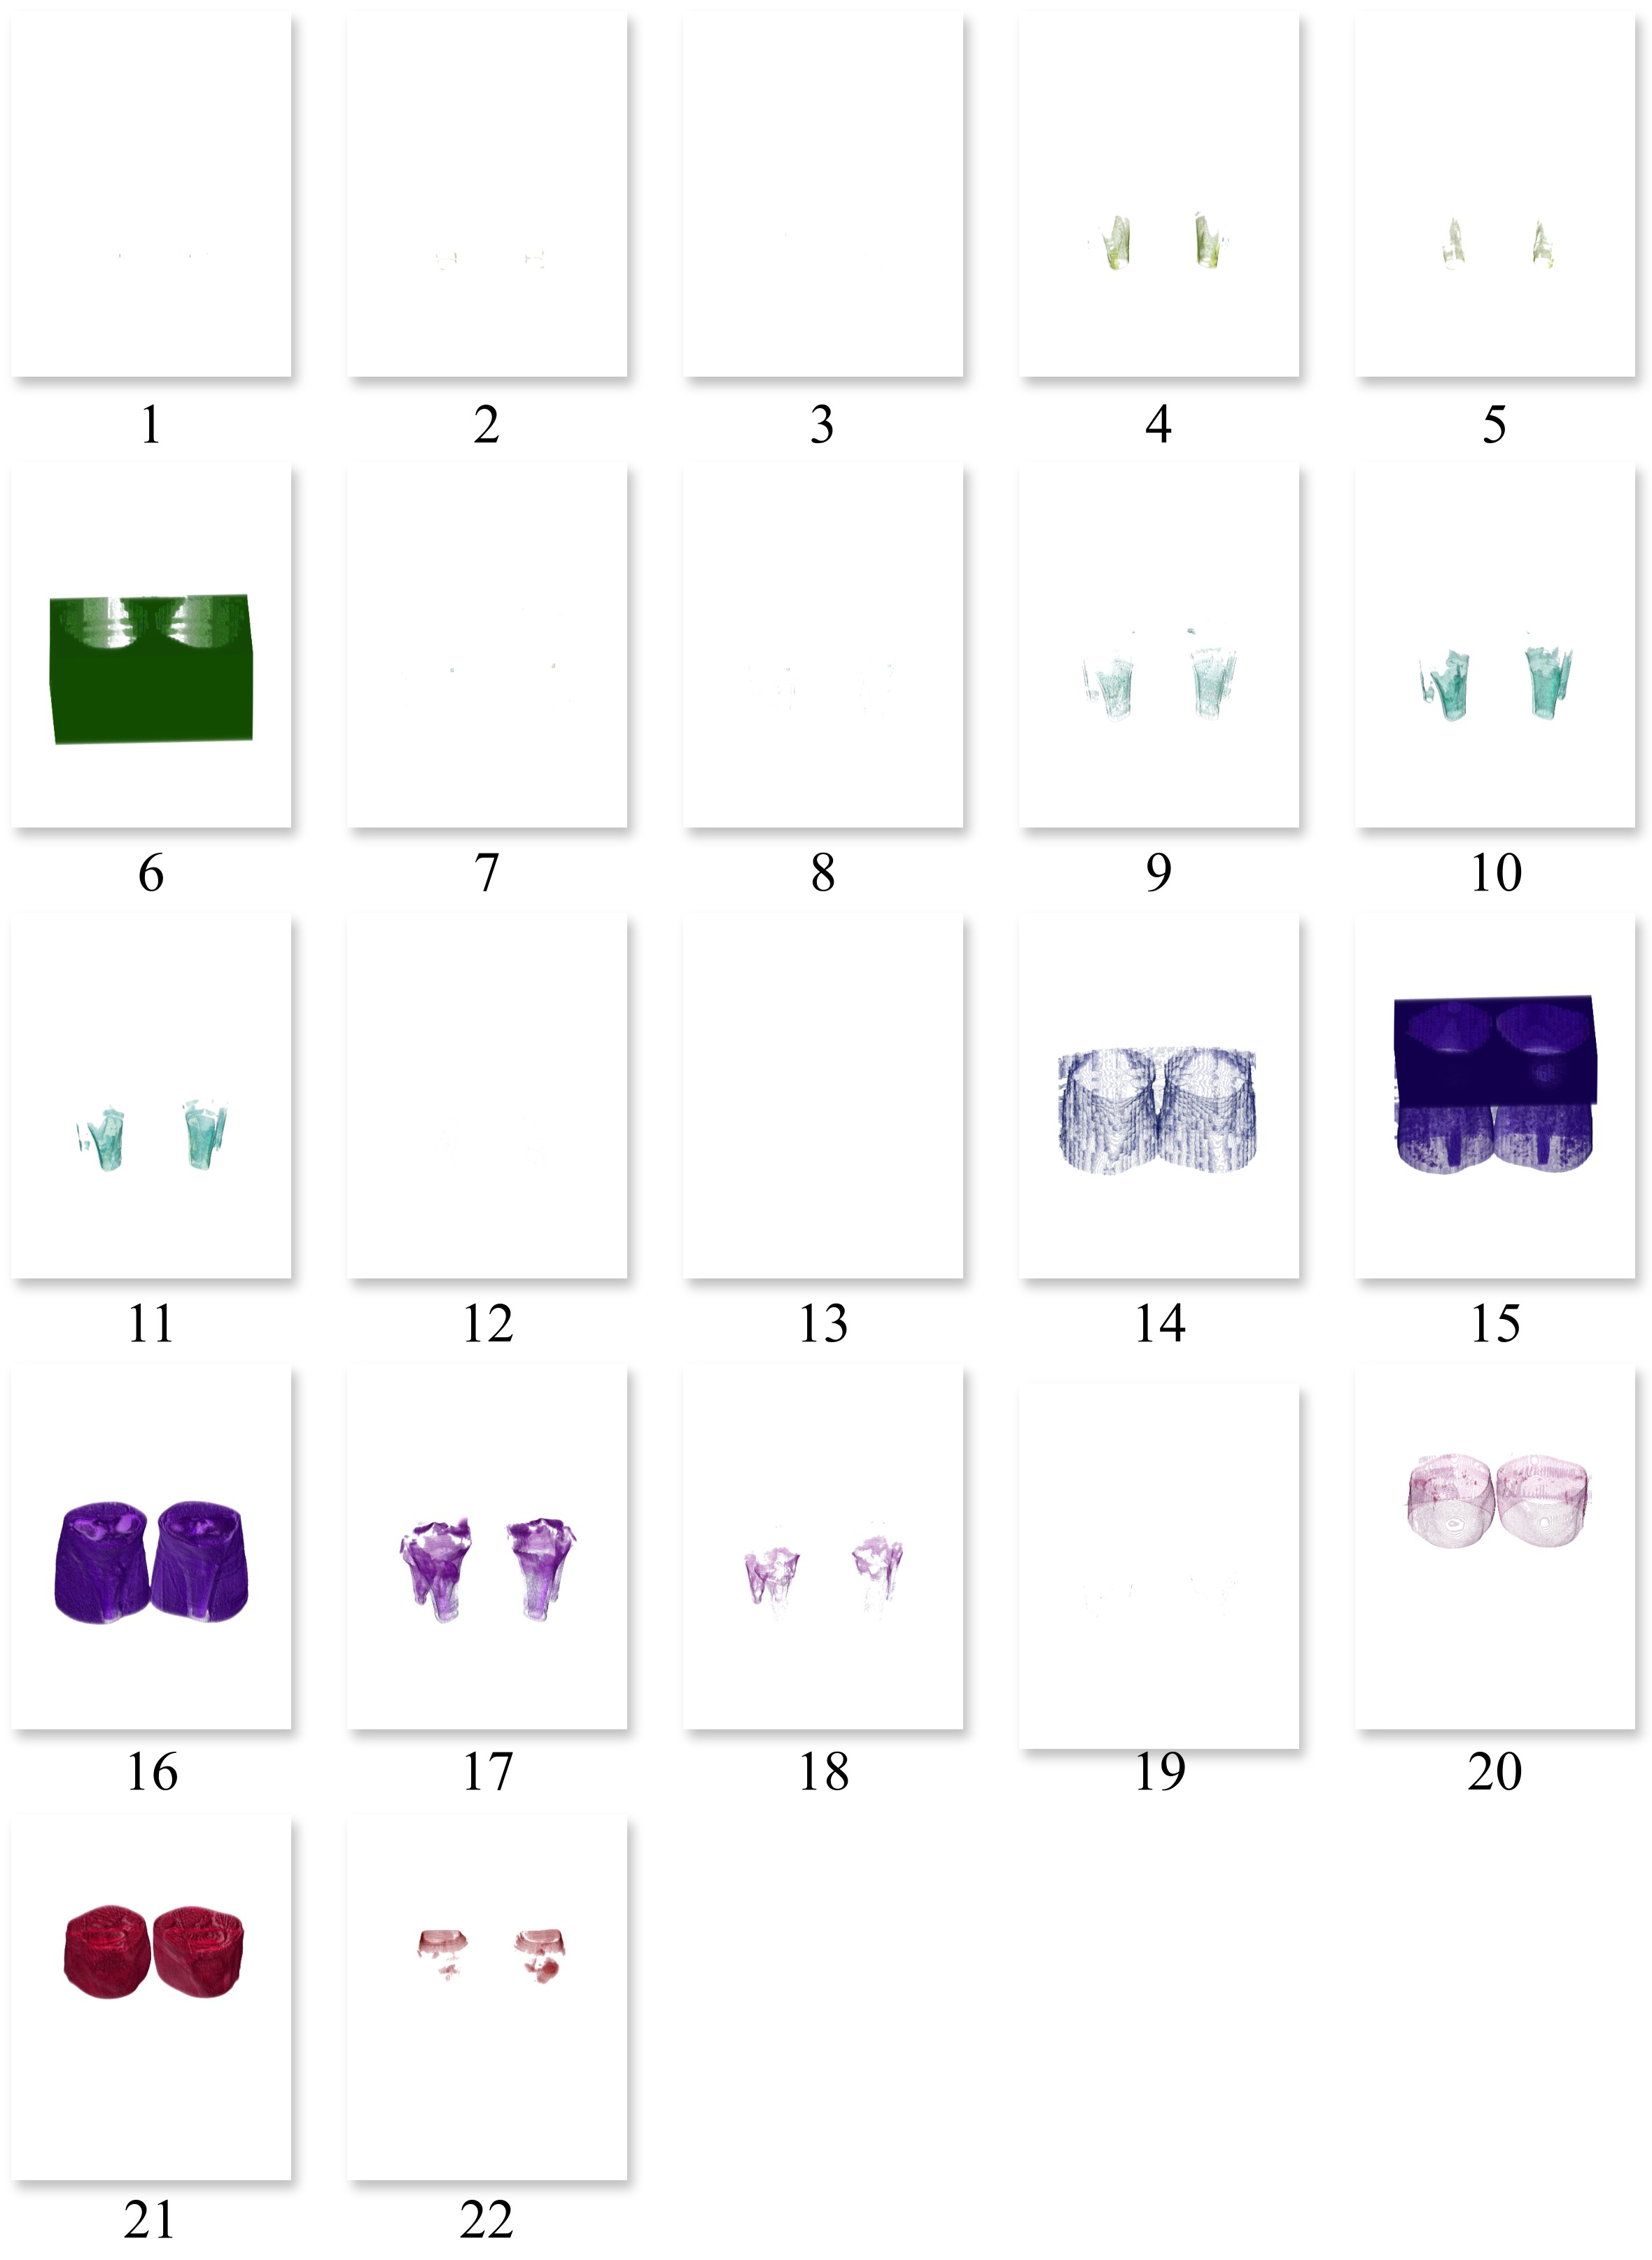
\includegraphics[width=\columnwidth]{figs/knees-clusters.jpg} 
    \caption{Rendered classified volume details for knees dataset. Parameters as above.}
    \label{fig:knees-clusters}
\end{figure}

Figure~\ref{fig:knees-groups} illustrates grouped bones and muscles: femur, tibia, patella, fibula, thigh and knee muscles.

\begin{figure}[htb!]
    \centering
    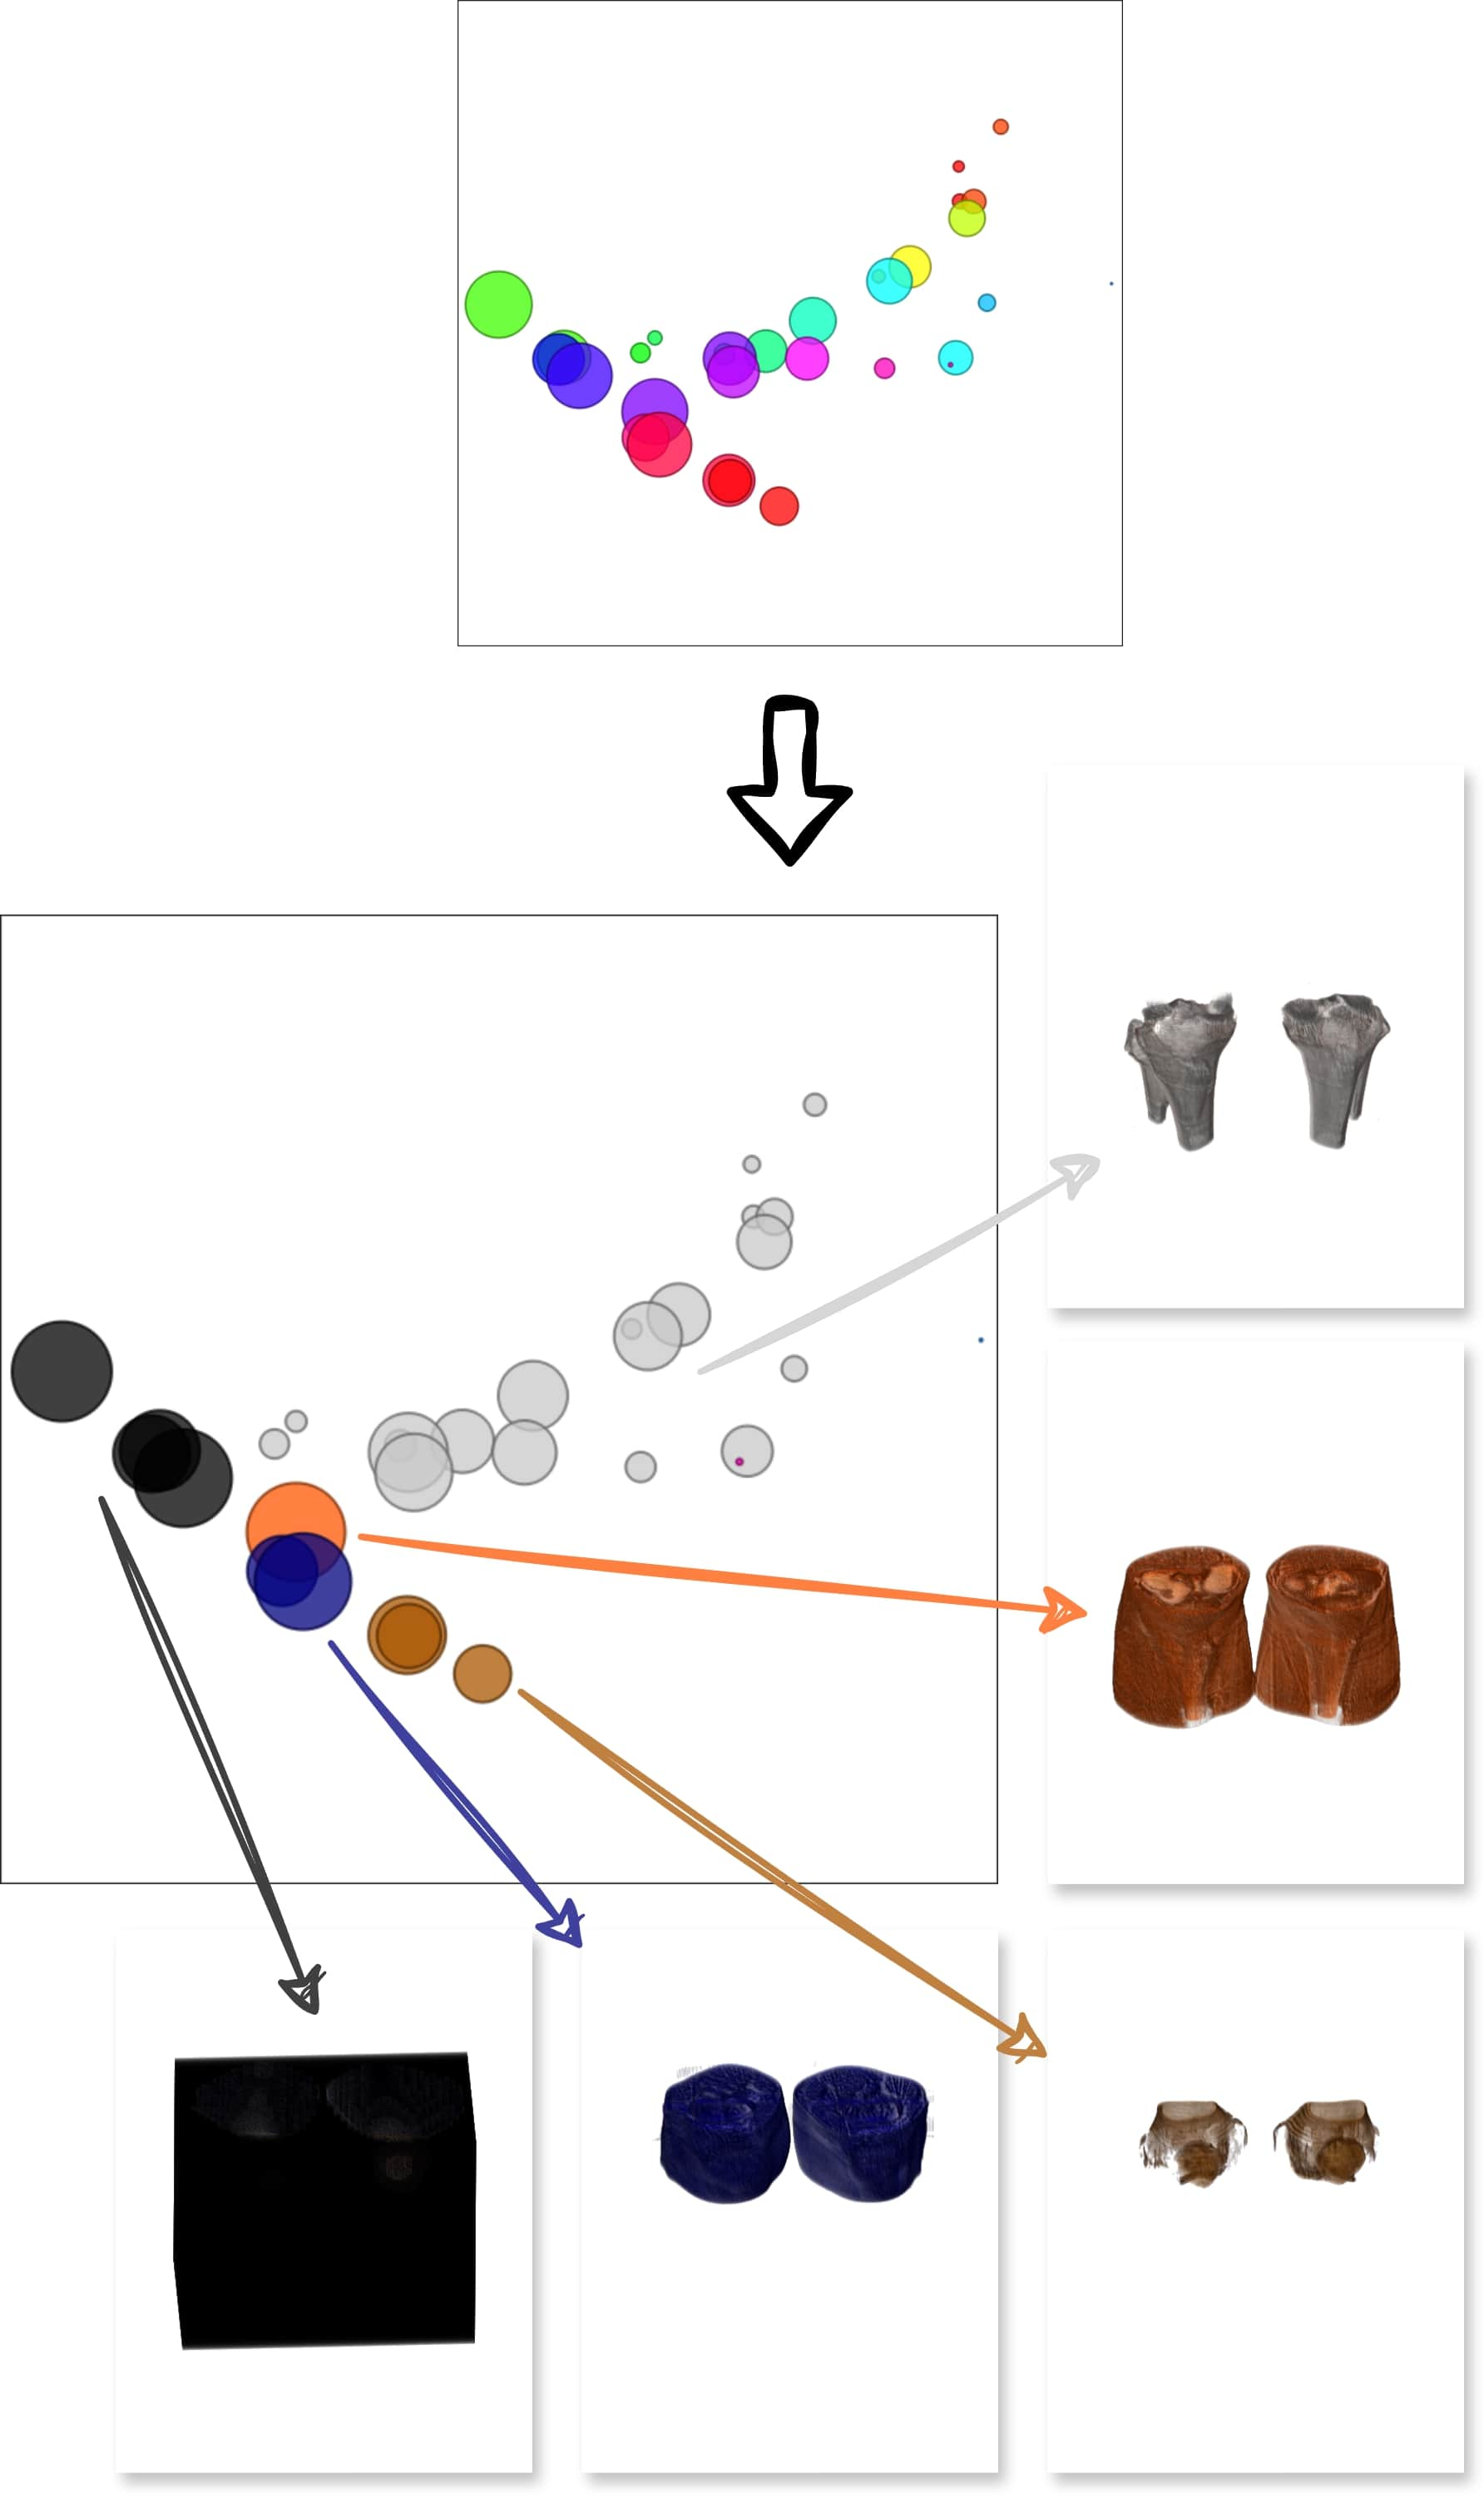
\includegraphics[width=\columnwidth]{figs/knees-groups.jpg}
    \caption{User-refined TF and classification for knees dataset. Groups formed empirically. Parameters as above.}
    \label{fig:knees-groups}
\end{figure}

\subsubsection{Tooth dataset}
\label{subsubsect:tooth-dataset}

Figure~\ref{fig:tooth-clusters} shows the volume exploration space, with rendered details in Fig.~\ref{fig:tooth-clusters}. Parameters: TF = \{intensity, variance, absolute deviation, energy, contrast, entropy\}; $minPts=4$; $\varepsilon=0.23$; $\alpha=0.9$.

\begin{figure}[htb!]
    \centering
    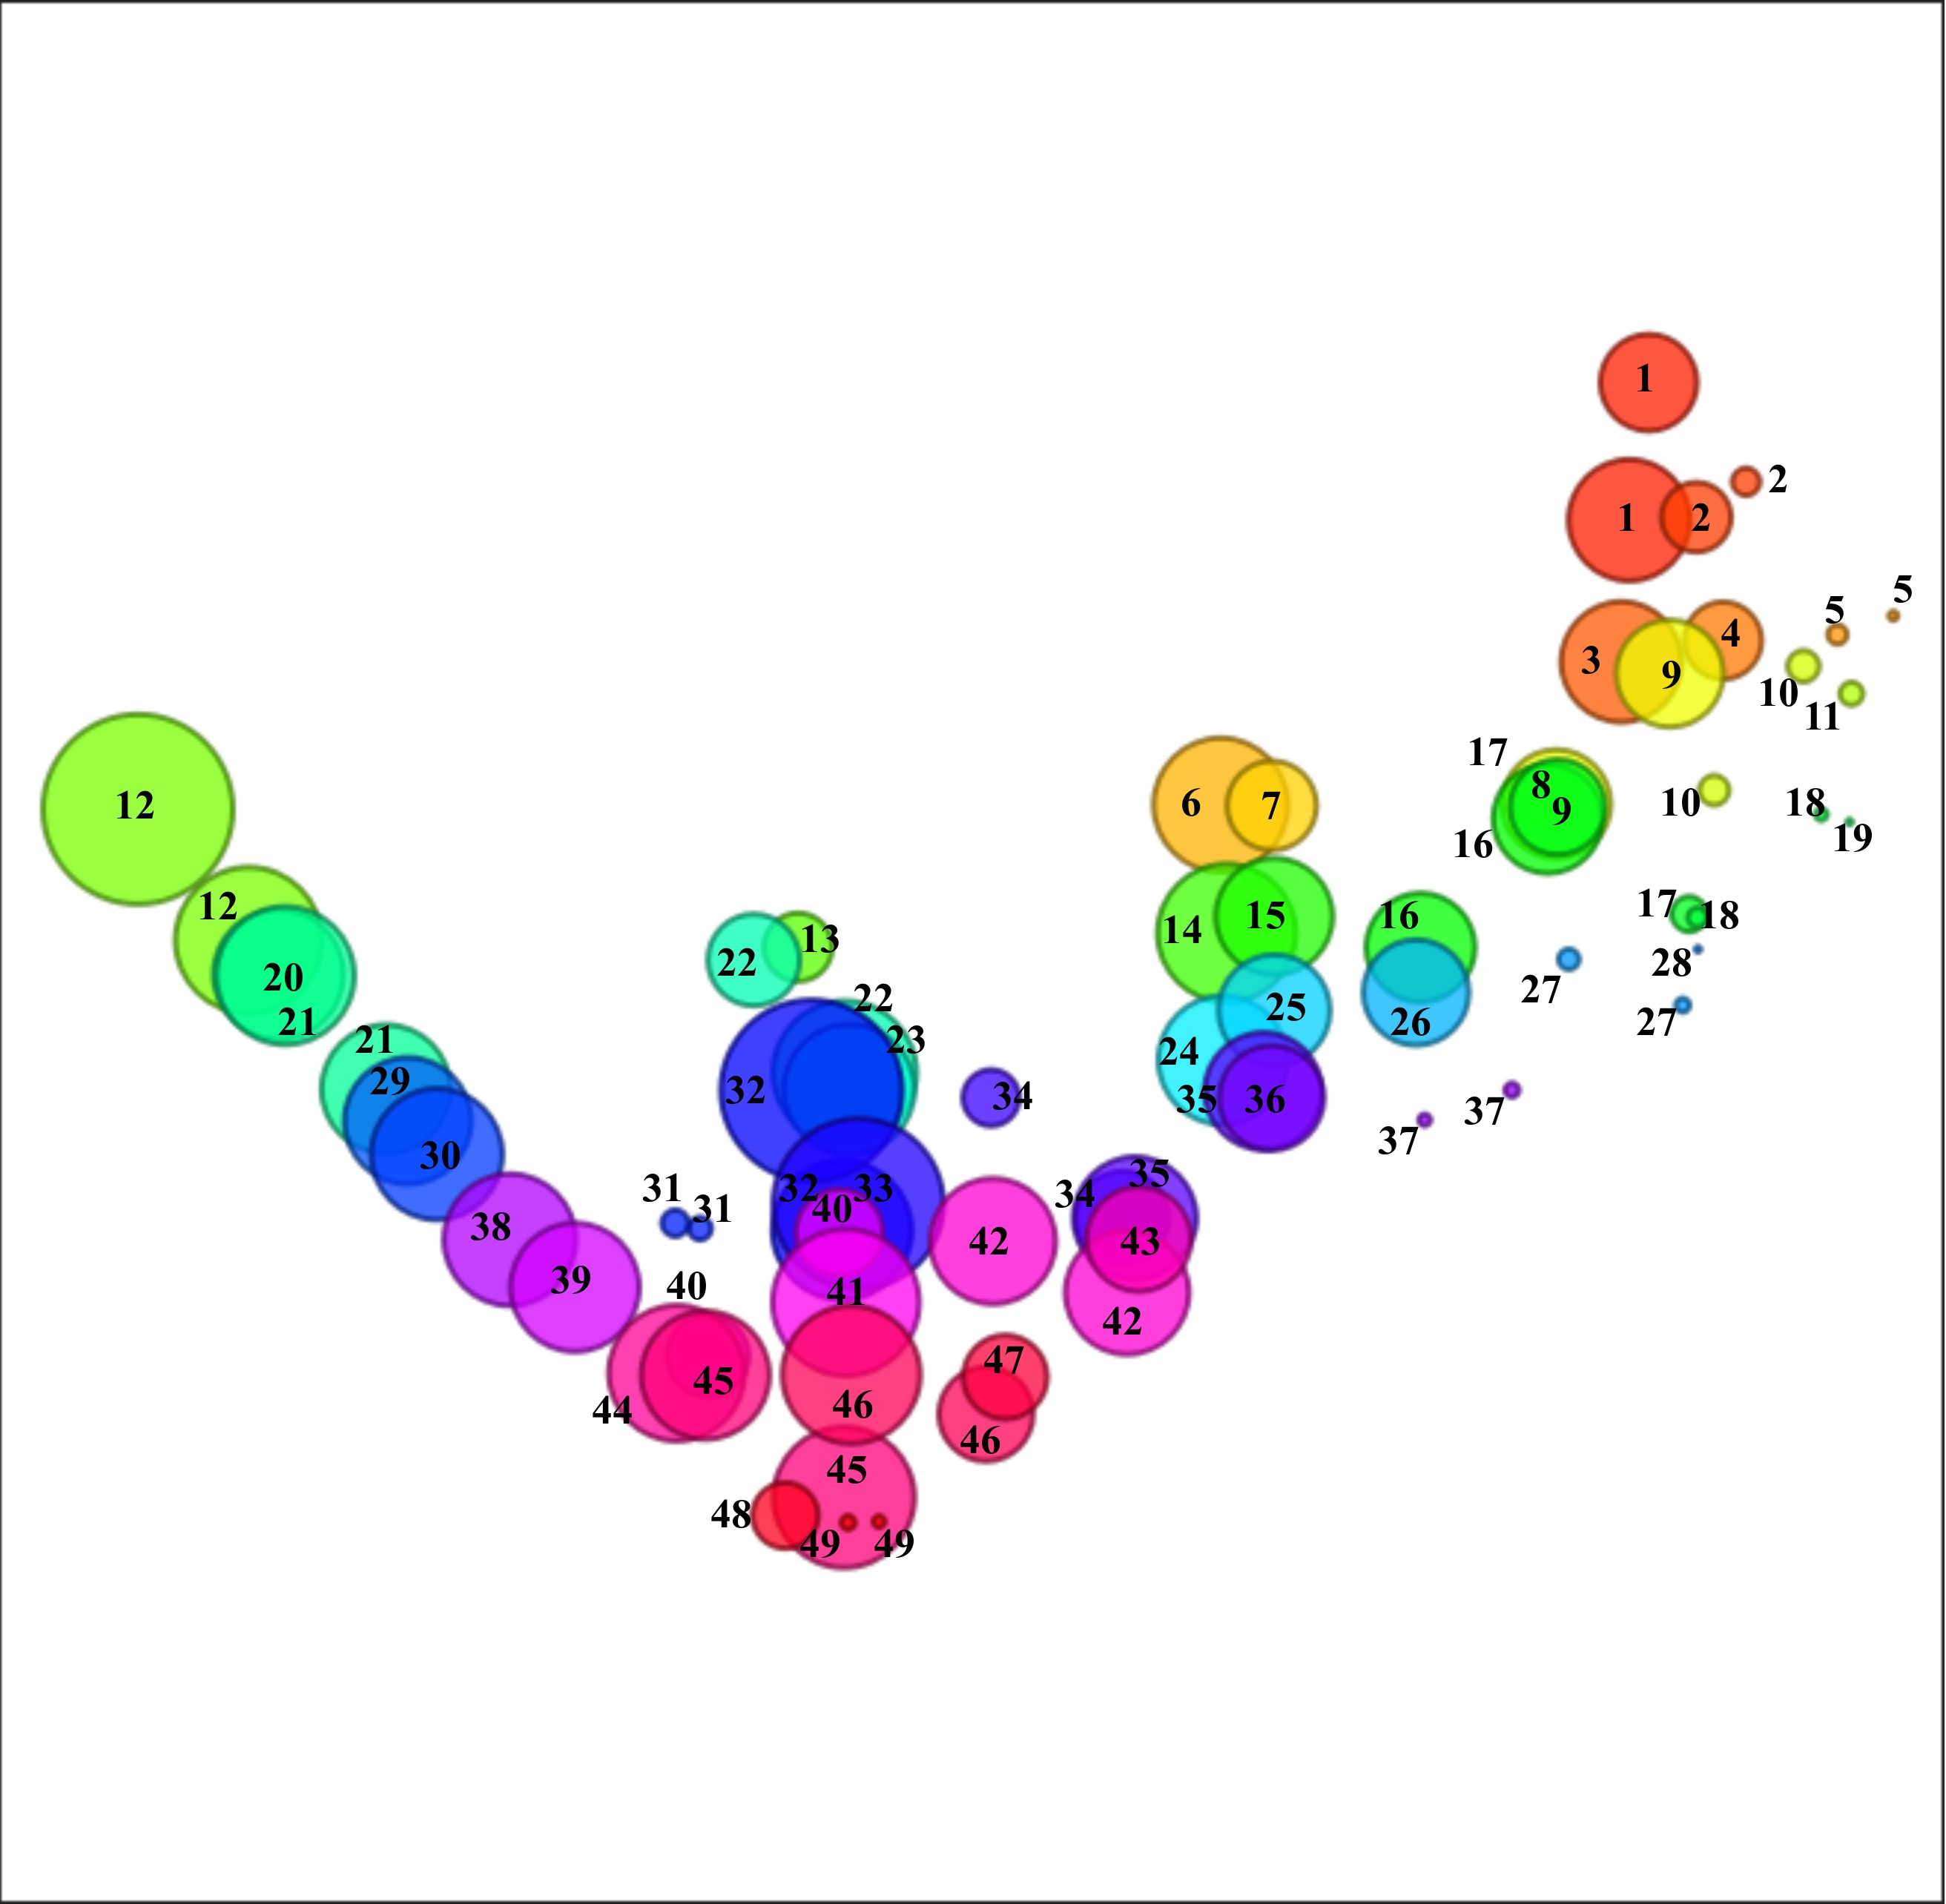
\includegraphics[width=0.7\columnwidth]{figs/tooth-clusters-tf.jpg} 
    \caption{Volume exploration space for tooth dataset. Parameters as above.}
    \label{fig:tooth-clusters}
\end{figure}

\begin{figure}[htb!]
    \centering
    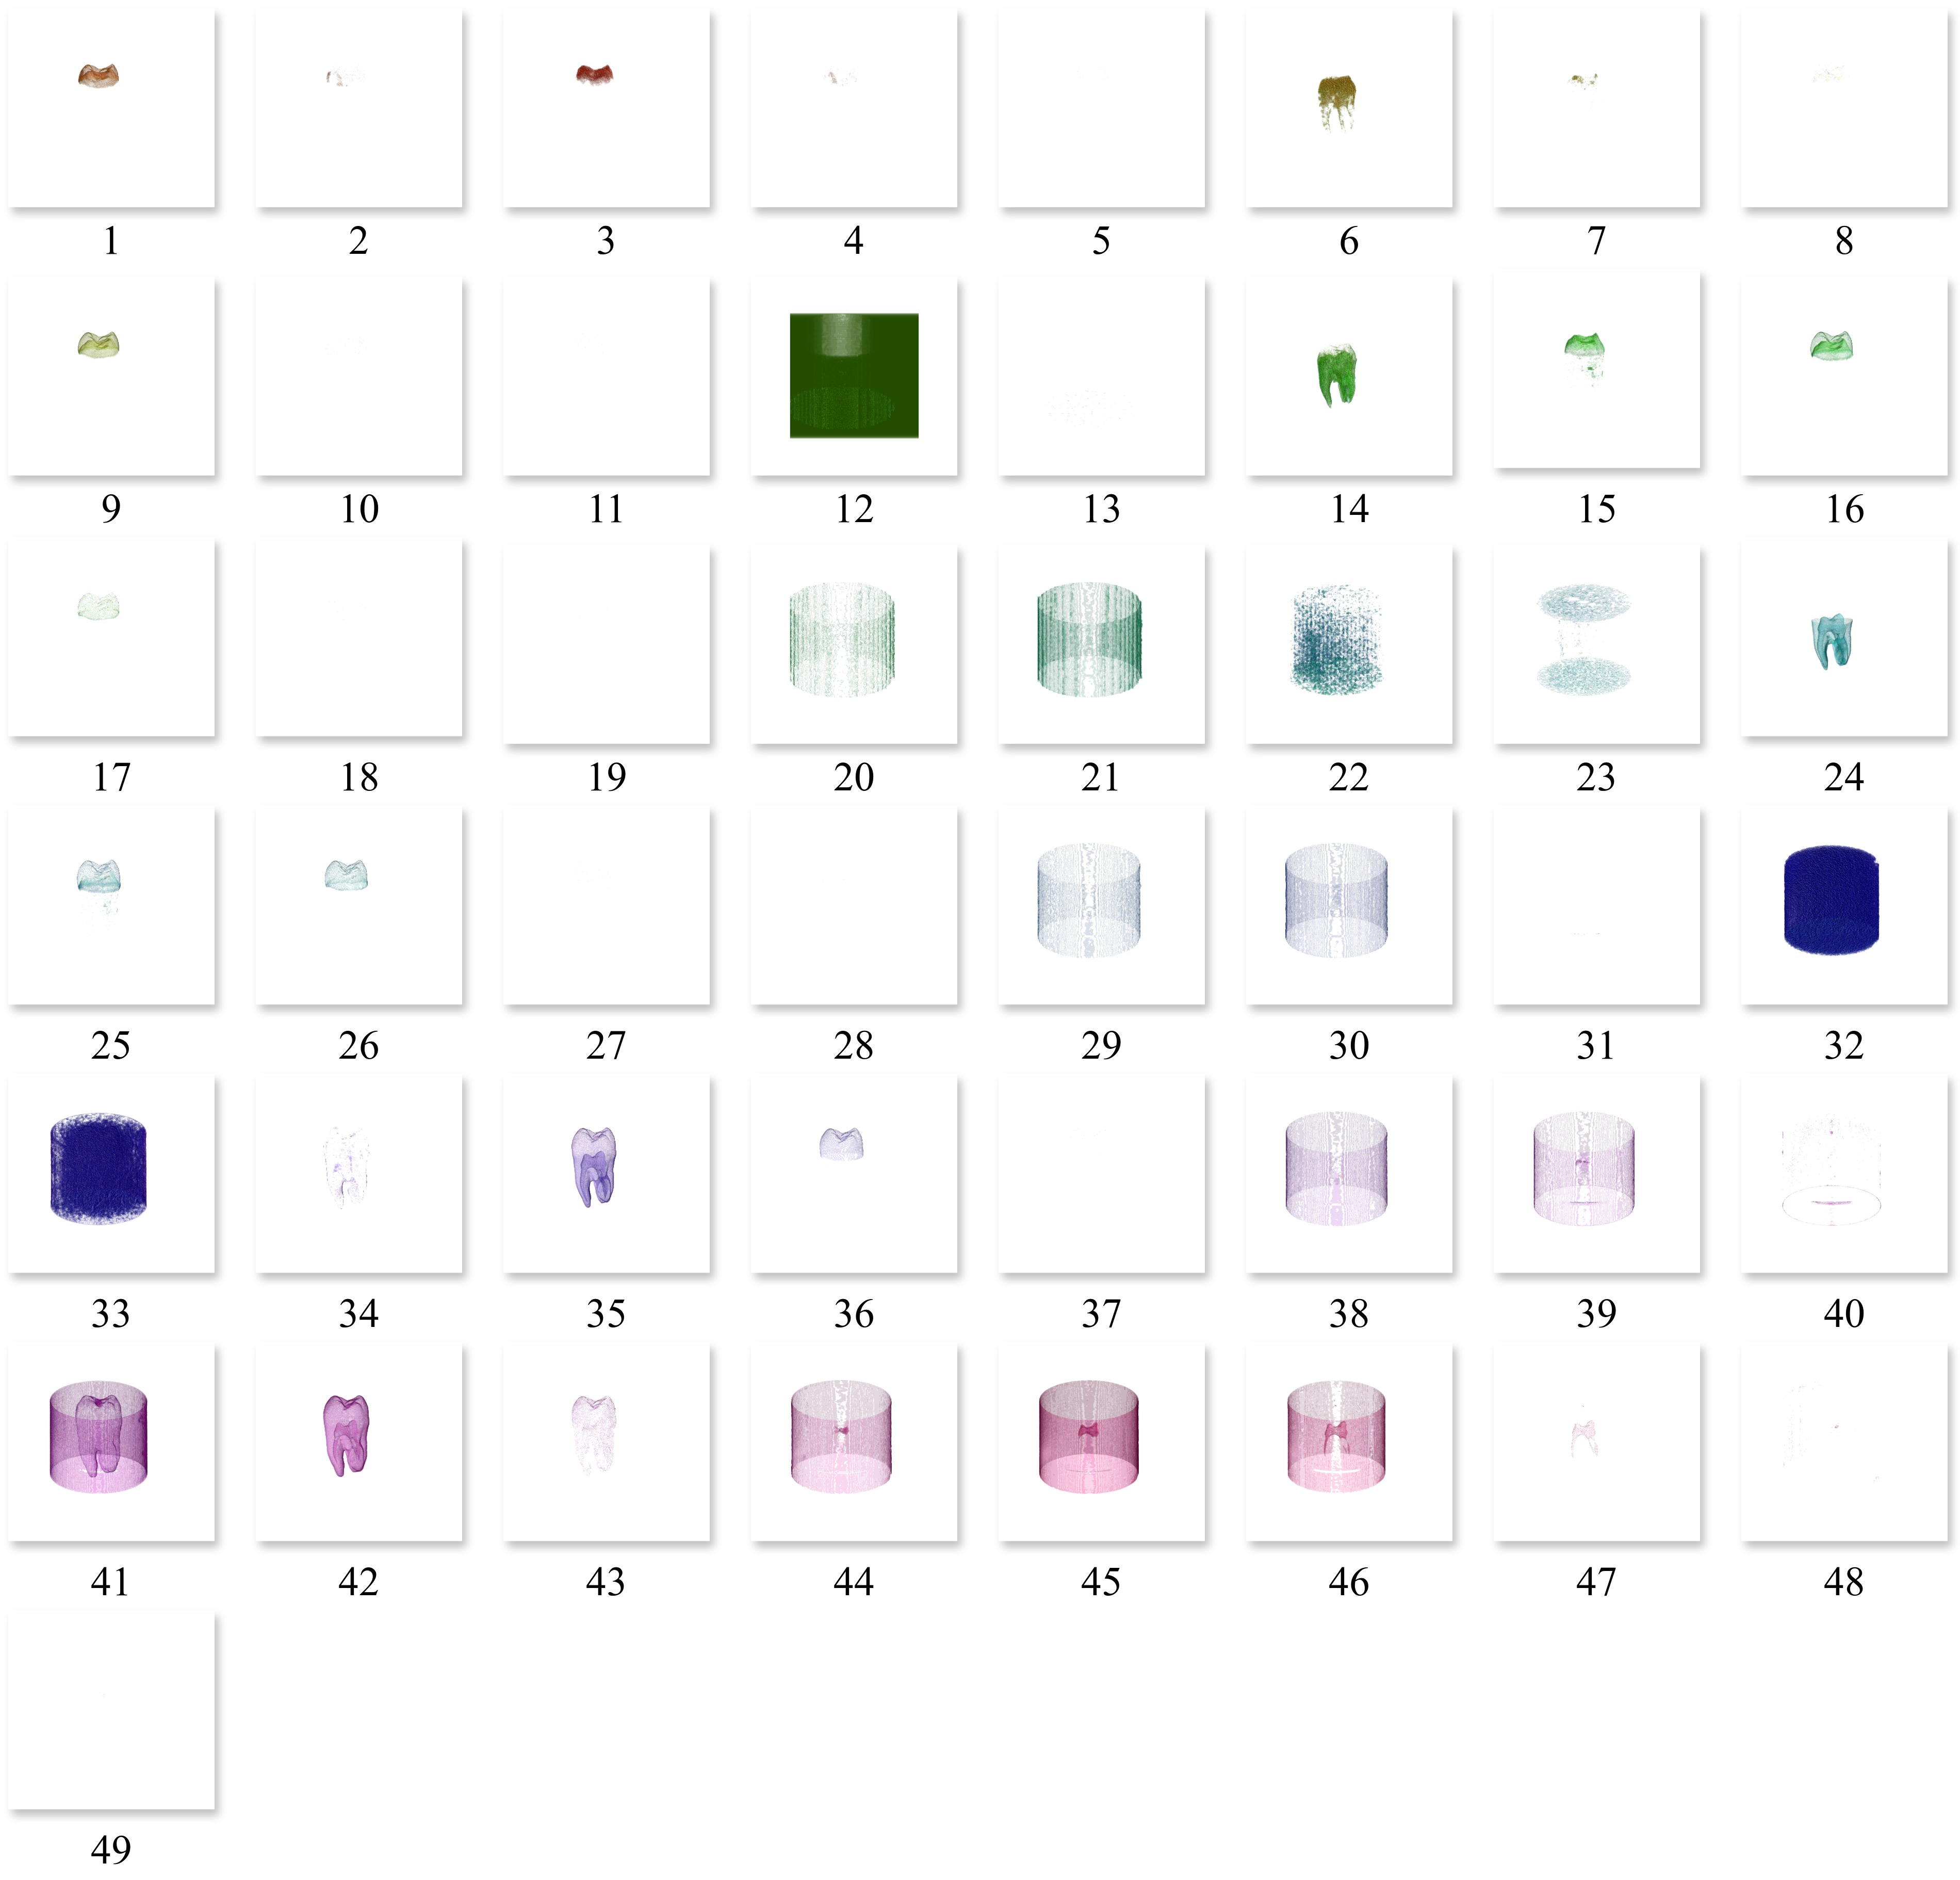
\includegraphics[width=\columnwidth]{figs/tooth-clusters.jpg} 
    \caption{Rendered classified volume details for tooth dataset. Parameters as above.}
    \label{fig:tooth-clusters}
\end{figure}

Figure~\ref{fig:tooth-groups} shows empirically grouped tooth structures: enamel, pulp, dentin, crown, entire tooth, and immersion fluid.

\begin{figure}[htb!]
    \centering
    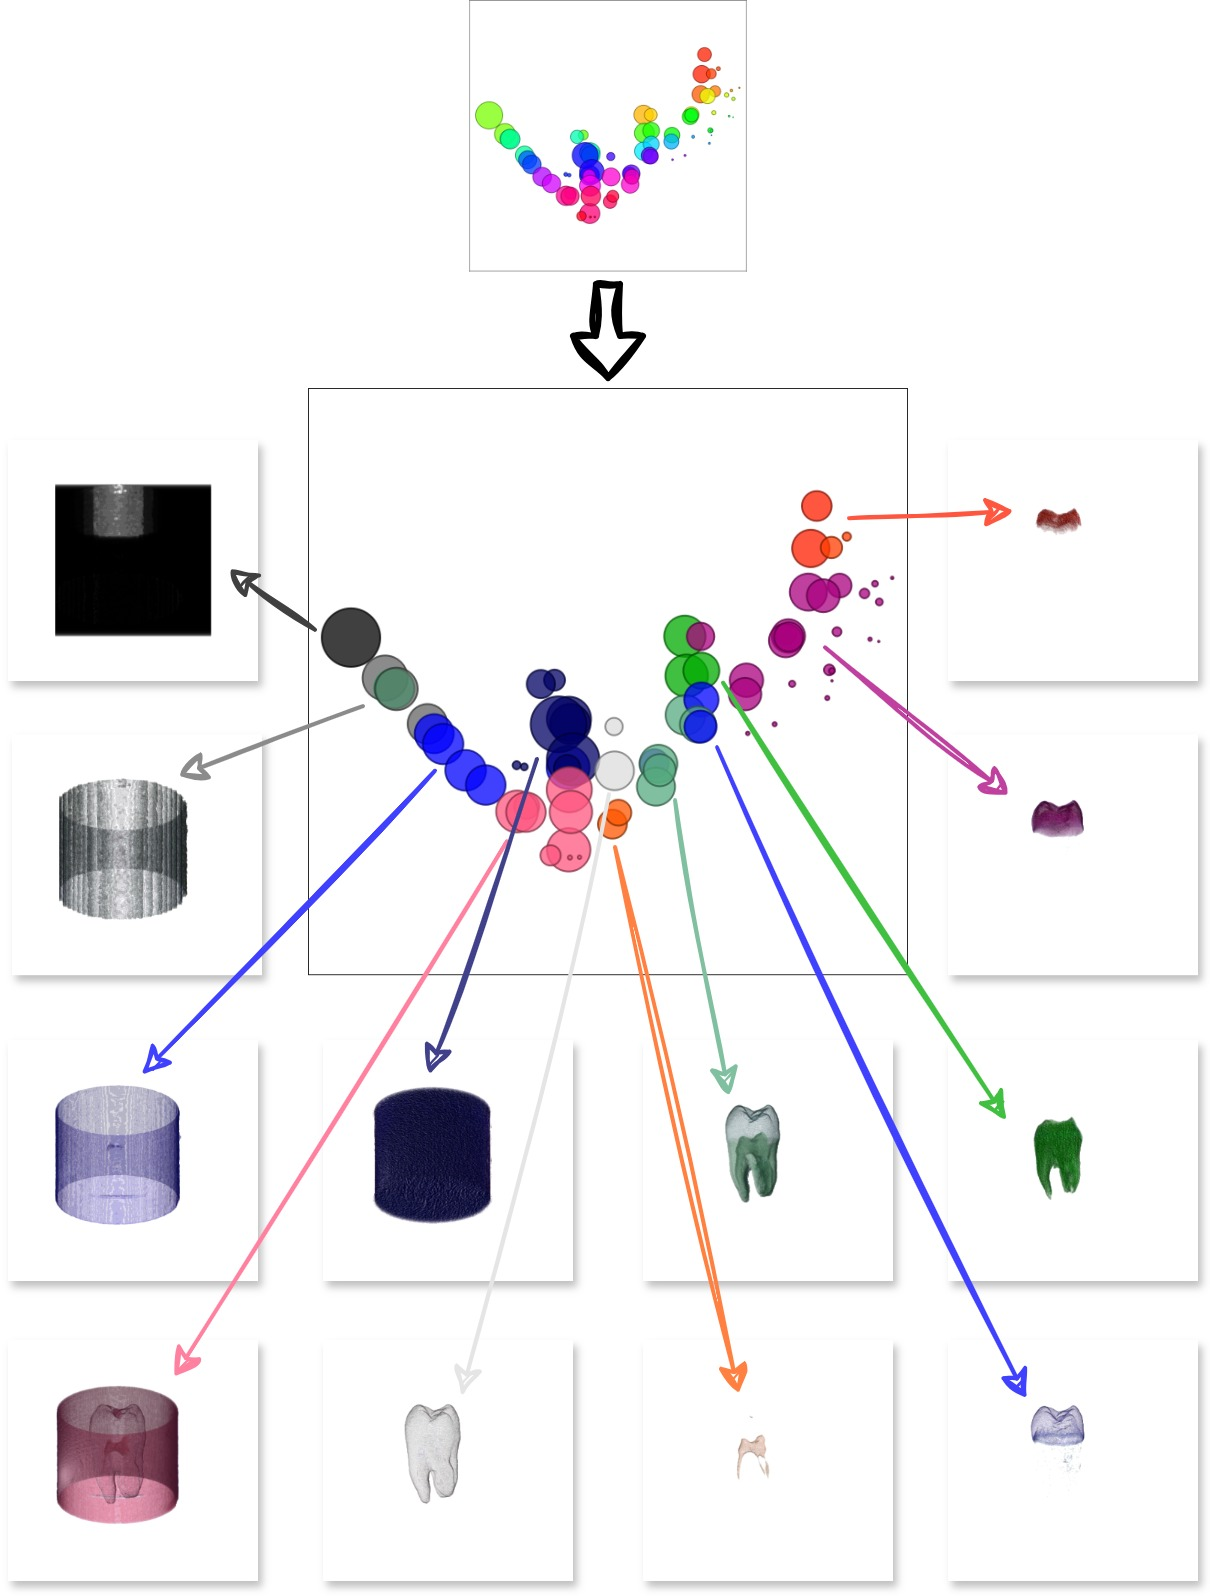
\includegraphics[width=\columnwidth]{figs/tooth-groups.jpg}
    \caption{User-refined TF and classification for tooth dataset. Groups formed empirically. Parameters as above.}
    \label{fig:tooth-groups}
\end{figure}
